\section{Experiment 3 - Adjusting Parameters}
\label{sec:exp3}
In this set of experiments the fitness functions $F_{basic}^{min}$ \eqref{eq:FBasicMin} and $F_{edge}^{min}$ \eqref{eq:FEdgeMin} are tested again on the Dataset1 (Experiment 3a and 3b) and the Healthcare dataset (Experiment 3c and 3d), but with an adjusted setup as shown in table \ref{tab:exp3_setup}. The setup is relaxing the objective for minimizing the role model complexity (role count, assignment counts).

\begin{table}[H]
    \centering
    \begin{adjustbox}{width=0.5\textwidth}
	    \begin{tabular}{|l|l|}
	        \hline
	        \rowcolor{myGray} 
	        \textbf{Parameter}              & \textbf{Value}    \\ \hline
	        Generations                     & 1000              \\ \hline
	        Population                      & 1000              \\ \hline
	        CXPB                            & 0.25              \\ \hline
	        MUTPB                           & 0.25              \\ \hline
	        MUTPB-Type1: Add role           & 0.5               \\ \hline
	        MUTPB-Type2: Add User           & 0.25              \\ \hline
	        MUTPB-Type3: Add Permission     & 0.25              \\ \hline
	        MUTPB-Type4: Remove Role        & 0.1               \\ \hline
	        MUTPB-Type5: Remove User        & 0.25              \\ \hline
	        MUTPB-Type6: Remove Permission  & 0.25              \\ \hline
	        Tournament size                 & 2                 \\ \hline
	        Local optimization              & True        		\\ \hline
	        Weights for Fitness Function    & 0.1, 1.0, 1.0     \\ \hline
	    \end{tabular}
	\end{adjustbox}
    \caption{EXPERIMENT 3 setup}
    \label{tab:exp3_setup}
\end{table}

The results can be seen in experiment 3a-d in table \ref{tab:exp2_results}. The results show that solutions with better fitness can be found by adjusting the parameters. One of the individuals with the best fitness solution of the experiments with the Healthcare dataset can be seen in Figure \ref{fig:exp3d_RM}. Examples of individuals with the best achieved fitness for the Dataset1 can be seen in the Appendix \ref{sec:A_Exp3a} and \ref{sec:A_Exp3b}.

There are many parameters, which can be adjusted and other settings might lead to even better results.

\begin{figure}[H]
    \centering
    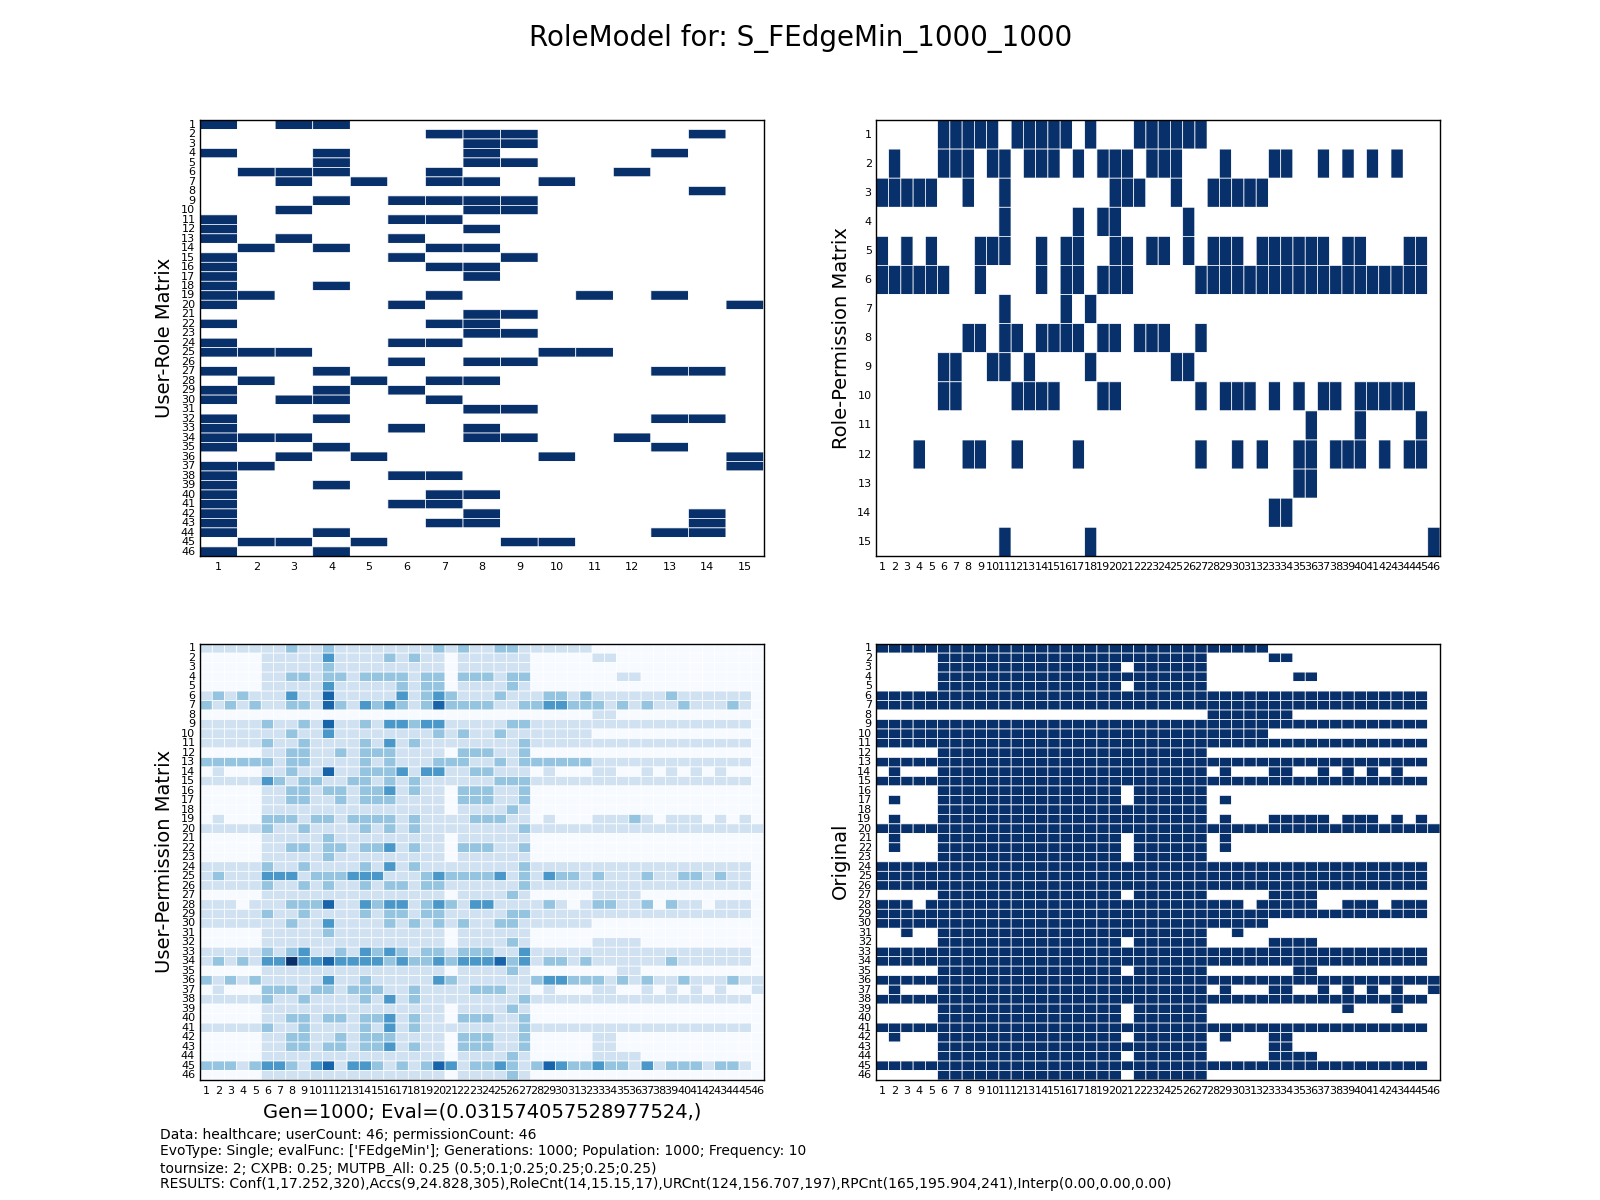
\includegraphics[width=\textwidth, trim=4cm 2cm 4cm 2cm, clip=true]{exp3d_RM}
    \caption{EXPERIMENT 3d: Example of role model resulting of Evo-RoleMiner with Fitness function $F_{edge}^{min}$ on the Healthcare dataset with setup in table \ref{tab:exp3_setup}. The role model has a role count of 14, one confidentiality violation, 23 availability violations, 152 user-role- and 192 role-permission-assignments. The fitness measure of the individual is 0.032. From u.l. to l.r.: User-Role Matrix, Role-Permission Matrix, Resulting User-Permission Matrix, Original User-Permission Matrix from Input. A blue box stands for an assignment. The darker the blue the more user-role- and role-permission assignments causing the user-permission assignment.}
    \label{fig:exp3d_RM}
\end{figure}

Another critical point is the diversity of the individuals in the populations in order to be able to find a perfect solution. When looking on the role count diversity it can be noted, that the individuals of a population quickly get the same role count size. The boxplot in Figure \ref{fig:exp3c_diversity} visualizes the role count diversity of the individuals in a population in different generations in one of the experiments. The boxplots in the other experiment look similar.

\begin{figure}[H]
	\centering
	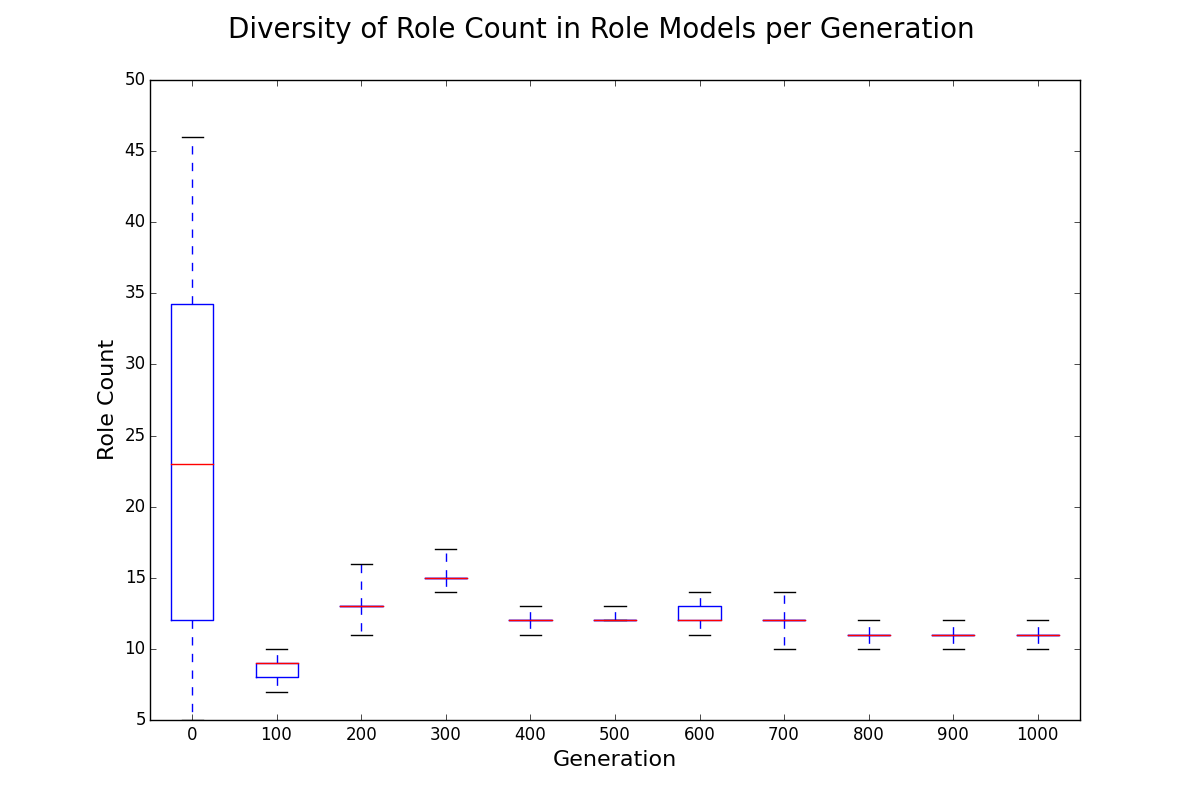
\includegraphics[width=0.7\textwidth]{exp3c_diversity}
	\caption{EXPERIMENT 3c: Example boxplot of role count diversity of individuals of a population in different generations. Experiment was executed on the Healthcare dataset.}
	\label{fig:exp3c_diversity}
\end{figure}

It is therefore not surprising that it is difficult for the Evo-RoleMiner to find an individual with a minimum amount of violations. Therefore the Evo-RoleMiner$M$ is tested in the next experiments.